% Chapter Template

\chapter{Ensayos y Resultados} % Main chapter title

\label{Chapter4} % Change X to a consecutive number; for referencing this chapter elsewhere, use \ref{ChapterX}

%----------------------------------------------------------------------------------------
%	SECTION 1
%----------------------------------------------------------------------------------------

%\section{Pruebas funcionales del hardware}
%\label{sec:pruebasHW}

%La idea de esta sección es explicar cómo se hicieron los ensayos, qué resultados se obtuvieron y analizarlos.

\section{Validación de grafos}
	
	\subsubsection{Topología bypass}
	\subsubsection{Topología playa de maniobras}
	\subsubsection{Topología estación}
			
\section{Validación del nodo}

	\subsection{Testbench del módulo nodo}
			
			Se generó el Algoritmo \ref{lst:test_nodo} para ...
			
			\begin{lstlisting}[language = vhdl,caption=Testbench del módulo nodo,label={lst:test_nodo}] 
				
					end;
			\end{lstlisting}
			
		\subsection{Resultados obtenidos}
			
			Figura \ref{fig:TEST_Nodo} ...
			
			\begin{figure}[h]
			\centering
			%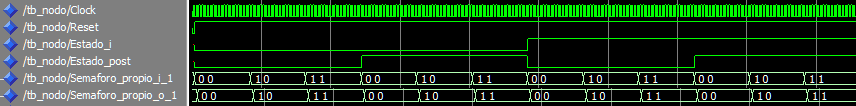
\includegraphics[scale=0.5]{./Figures/Test/Nodo}
				\caption{Simulación de un nodo}
				\label{fig:Test_Nodo}
			\end{figure}
				
			blabla
			
	
\section{Validación de la máquina de cambios}

	\subsection{Testbench del módulo de la máquina de cambios}
			
		Se generó el Algoritmo \ref{lst:test_cambios} para ...
			
		\begin{lstlisting}[language = vhdl,caption=Testbench del módulo de la máquina de cambios,label={lst:test_cambios}] 
				
			end;
		\end{lstlisting}
			
	\subsection{Resultados obtenidos}
			
		Figura \ref{fig:TEST_Cambios} ...
		
		\begin{figure}[h]
		\centering
		%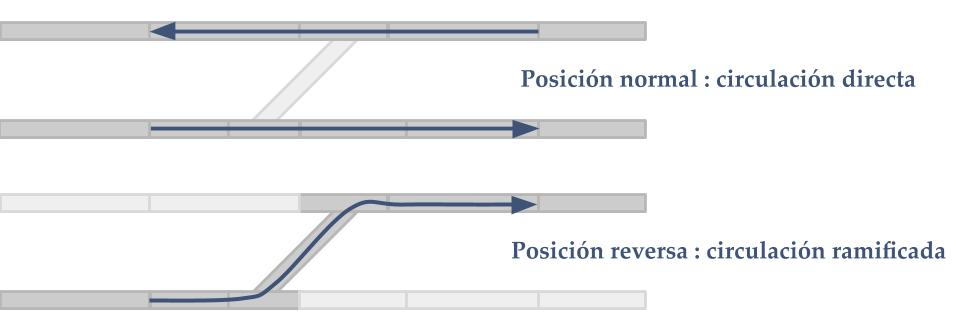
\includegraphics[scale=0.5]{./Figures/Test/Cambios}
			\caption{Simulación de la máquina de cambios}
			\label{fig:Test_Cambios}
		\end{figure}
			
		blabla
			
\section{Validación de la UART}

	\subsection{Testbench del módulo UART}
			
		Se generó el Algoritmo \ref{lst:test_uart} para ...
		
		Detector + Switch abajo + Registro
			
		\begin{lstlisting}[language = vhdl,caption=Testbench del módulo UART,label={lst:test_uart}] 
				
			end;
		\end{lstlisting}
			
	\subsection{Resultados obtenidos}
		
		
			
		Figura \ref{fig:TEST_Uart} ...
		
		\begin{figure}[h]
		\centering
		%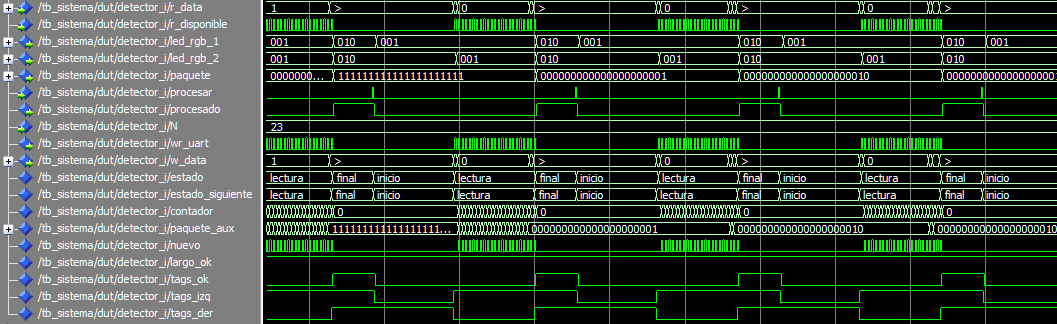
\includegraphics[scale=0.5]{./Figures/Test/Detector}
			\caption{Simulación de la UART}
			\label{fig:Test_UART}
		\end{figure}
			
		blabla
		
	
\section{Validación del detector}

	\subsection{Testbench del módulo detector}
			
		Se generó el Algoritmo \ref{lst:test_detector} para ...
		
			
		\begin{lstlisting}[language = vhdl,caption=Testbench del módulo detector,label={lst:test_detector}] 
				
			end;
		\end{lstlisting}
			
	\subsection{Resultados obtenidos}
				
		Figura \ref{fig:TEST_Detector} ...
		
		\begin{figure}[h]
		\centering
		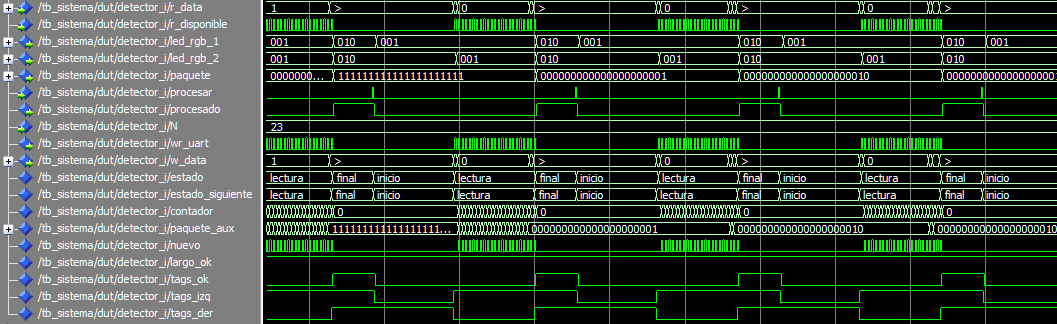
\includegraphics[scale=0.5]{./Figures/Test/Detector}
			\caption{Simulación del detector}
			\label{fig:Test_Detector}
		\end{figure}
	
\section{Validación del separador}

	\subsection{Testbench del módulo separador}
			
		Se generó el Algoritmo \ref{lst:test_separador} para ...
		
			
		\begin{lstlisting}[language = vhdl,caption=Testbench del módulo separador,label={lst:test_separador}] 
				
			end;
		\end{lstlisting}
			
	\subsection{Resultados obtenidos}
				
		Figura \ref{fig:TEST_Separador} ...
		
		\begin{figure}[h]
		\centering
		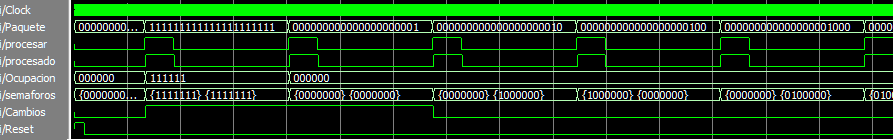
\includegraphics[scale=0.6]{./Figures/Test/Separador}
			\caption{Simulación del separador}
			\label{fig:Test_Separador}
		\end{figure}
		
\section{Validación del mediador}

	\subsection{Testbench del módulo mediador}
			
		Se generó el Algoritmo \ref{lst:test_mediador} para ...
		
			
		\begin{lstlisting}[language = vhdl,caption=Testbench del módulo mediador,label={lst:test_mediador}] 
				
			end;
		\end{lstlisting}
			
	\subsection{Resultados obtenidos}
				
		Figura \ref{fig:TEST_Mediador} ...
		
		\begin{figure}[h]
		\centering
		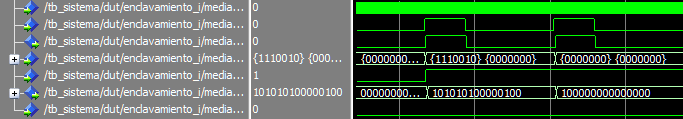
\includegraphics[scale=0.8]{./Figures/Test/Mediador}
			\caption{Simulación del mediador}
			\label{fig:Test_Mediador}
		\end{figure}
		
\section{Validación del enclavamiento}
	
	\subsection{Testbench del módulo enclavamiento}
			
		Se generó el Algoritmo \ref{lst:test_enclavamiento} para ...
		
			
		\begin{lstlisting}[language = vhdl,caption=Testbench del módulo enclavamiento,label={lst:test_enclavamiento}] 
				
			end;
		\end{lstlisting}
			
	\subsection{Resultados obtenidos}
				
		Figura \ref{fig:TEST_Enclavamiento} ...
		
		\begin{figure}[h]
		\centering
		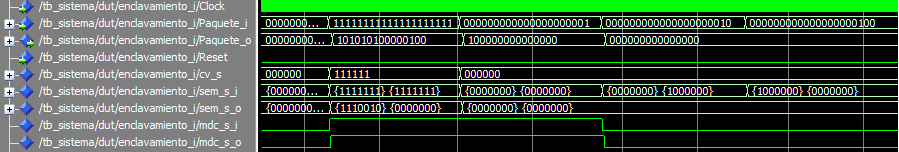
\includegraphics[scale=0.65]{./Figures/Test/Enclavamiento}
			\caption{Simulación del enclavamiento}
			\label{fig:Test_Enclavamiento}
		\end{figure}
	
\section{Validación del registro}

	\subsection{Testbench del módulo registro}
			
		Se generó el Algoritmo \ref{lst:test_registro} para ...
		
			
		\begin{lstlisting}[language = vhdl,caption=Testbench del módulo registro,label={lst:test_registro}] 
				
			end;
		\end{lstlisting}
			
	\subsection{Resultados obtenidos}
				
		Figura \ref{fig:TEST_Registro} ...
		
	\begin{figure}[h]
	\centering
	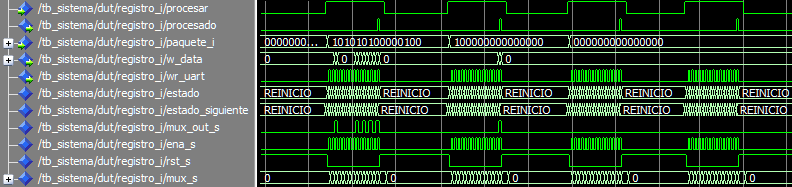
\includegraphics[scale=0.7]{./Figures/Test/Registro}
		\caption{Simulación del registro}
		\label{fig:Test_Registro}
	\end{figure}
	
\section{Validación del selector}

	\subsection{Testbench del módulo selector}
			
		Se generó el Algoritmo \ref{lst:test_selector} para ...
		
			
		\begin{lstlisting}[language = vhdl,caption=Testbench del módulo selector,label={lst:test_selector}] 
				
			end;
		\end{lstlisting}
			
	\subsection{Resultados obtenidos}
				
		Figura \ref{fig:TEST_Selector} ...
		
	\begin{figure}[h]
	\centering
	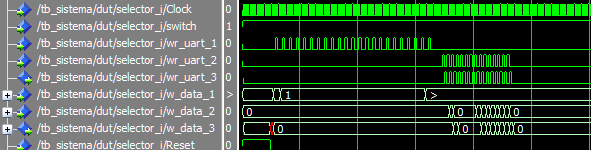
\includegraphics[scale=0.95]{./Figures/Test/Selector}
		\caption{Simulación del selector}
		\label{fig:Test_Selector}
	\end{figure}
			